\section{Enhancing images with edges}
\label{sec:enhancing}

Our function is capable of playing the video and overlap the detected edges.
For this exercise we have embedded some UI controls, so the user can change the edge
detection method and its parameters while the video is being shown. Some examples are
shown in figures \ref{fig:cannyvideobeach}, \ref{fig:sobelvideobeach},
\ref{fig:cannyvideocottage} and \ref{fig:cannyvideocottage}.

For this exercise we have decided to load frame after frame, process it and then
show the image with the overlapped edges. The idea behind this is to bound the
usage of memory. Therefore the relevance of the efficiency of the detectors came
into play. We have added to our method the functionality of displaying the mean time
between consecutive frames. For very slow detectors (Canny) the reproduction of the video was
to slow (the time between frames was greater than 160ms in a 1.8GHz computer) while with
less sophisticated detectors like Sobel the execution was considerably more agile (time
between frames lower than 70ms). This has to be taken into account in real-time applications
(e.g. in robotics).

\begin{figure}[!hbt]
  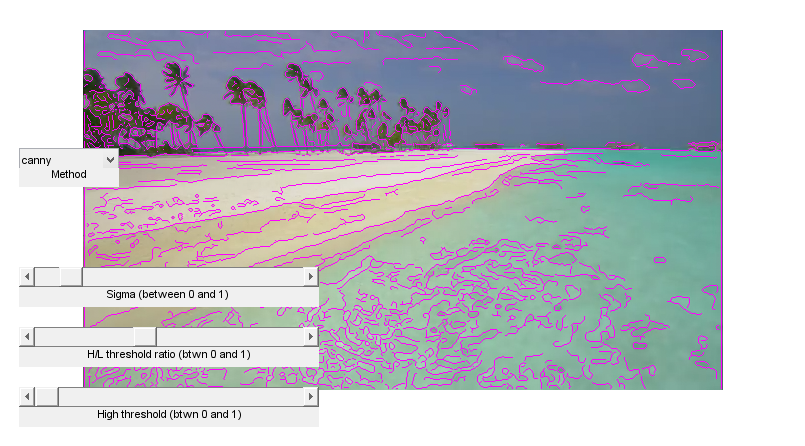
\includegraphics[width=\textwidth]{./img/ex2/frame_canny_1.png}
  \caption{Beach with overlapped edges (Canny)}
  \label{fig:cannyvideobeach}
\end{figure}

\begin{figure}[!hbt]
  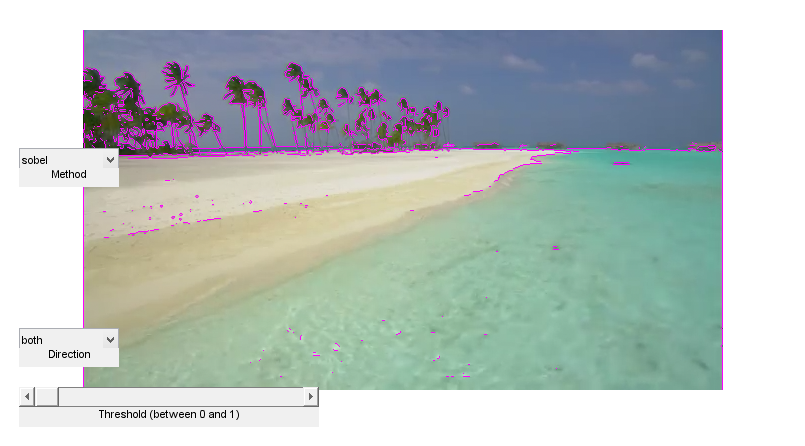
\includegraphics[width=\textwidth]{./img/ex2/frame_sobel_1.png}
  \caption{Beach with overlapped edges (Sobel)}
  \label{fig:sobelvideobeach}
\end{figure}

\begin{figure}[!hbt]
  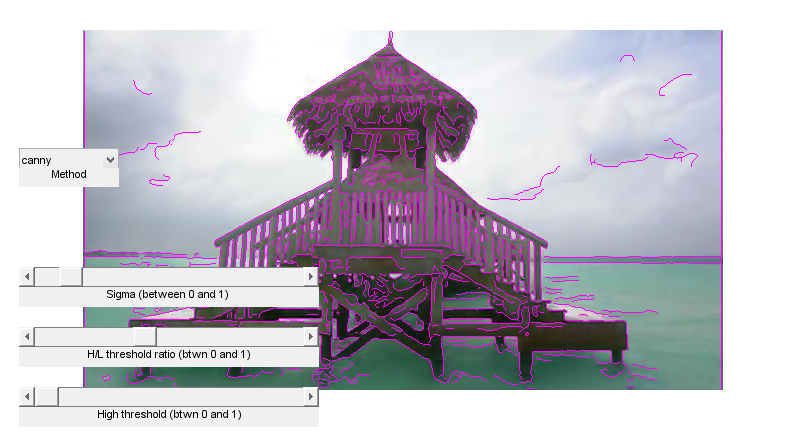
\includegraphics[width=\textwidth]{./img/ex2/frame_canny_2.png}
  \caption{Cottage with overlapped edges (Canny)}
  \label{fig:cannyvideocottage}
\end{figure}

\begin{figure}[!hbt]
  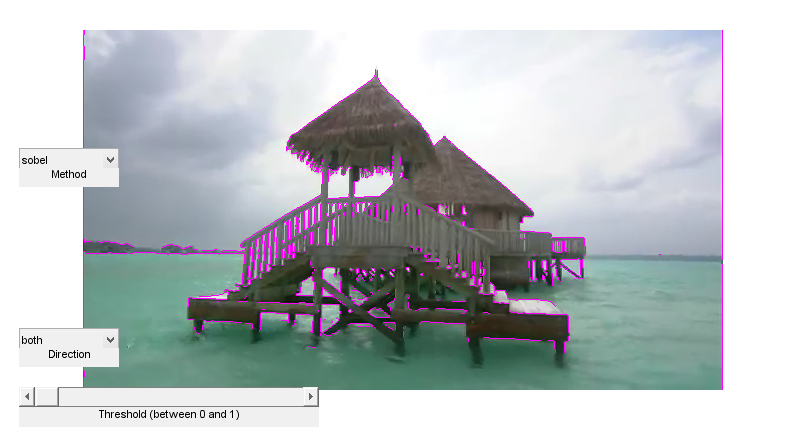
\includegraphics[width=\textwidth]{./img/ex2/frame_sobel_2.png}
  \caption{Cottage with overlapped edges (Sobel)}
  \label{fig:sobelvideocottage}
\end{figure}

For illustration purposes, we have selected three frames from the video and extracted their
edges using all the detectors but the simplest one. The comparisons are shown in figures
\ref{fig:firstcomparison}, \ref{fig:secondcomparison} and \ref{fig:thirdcomparison}.

\begin{figure}[!hbt]
  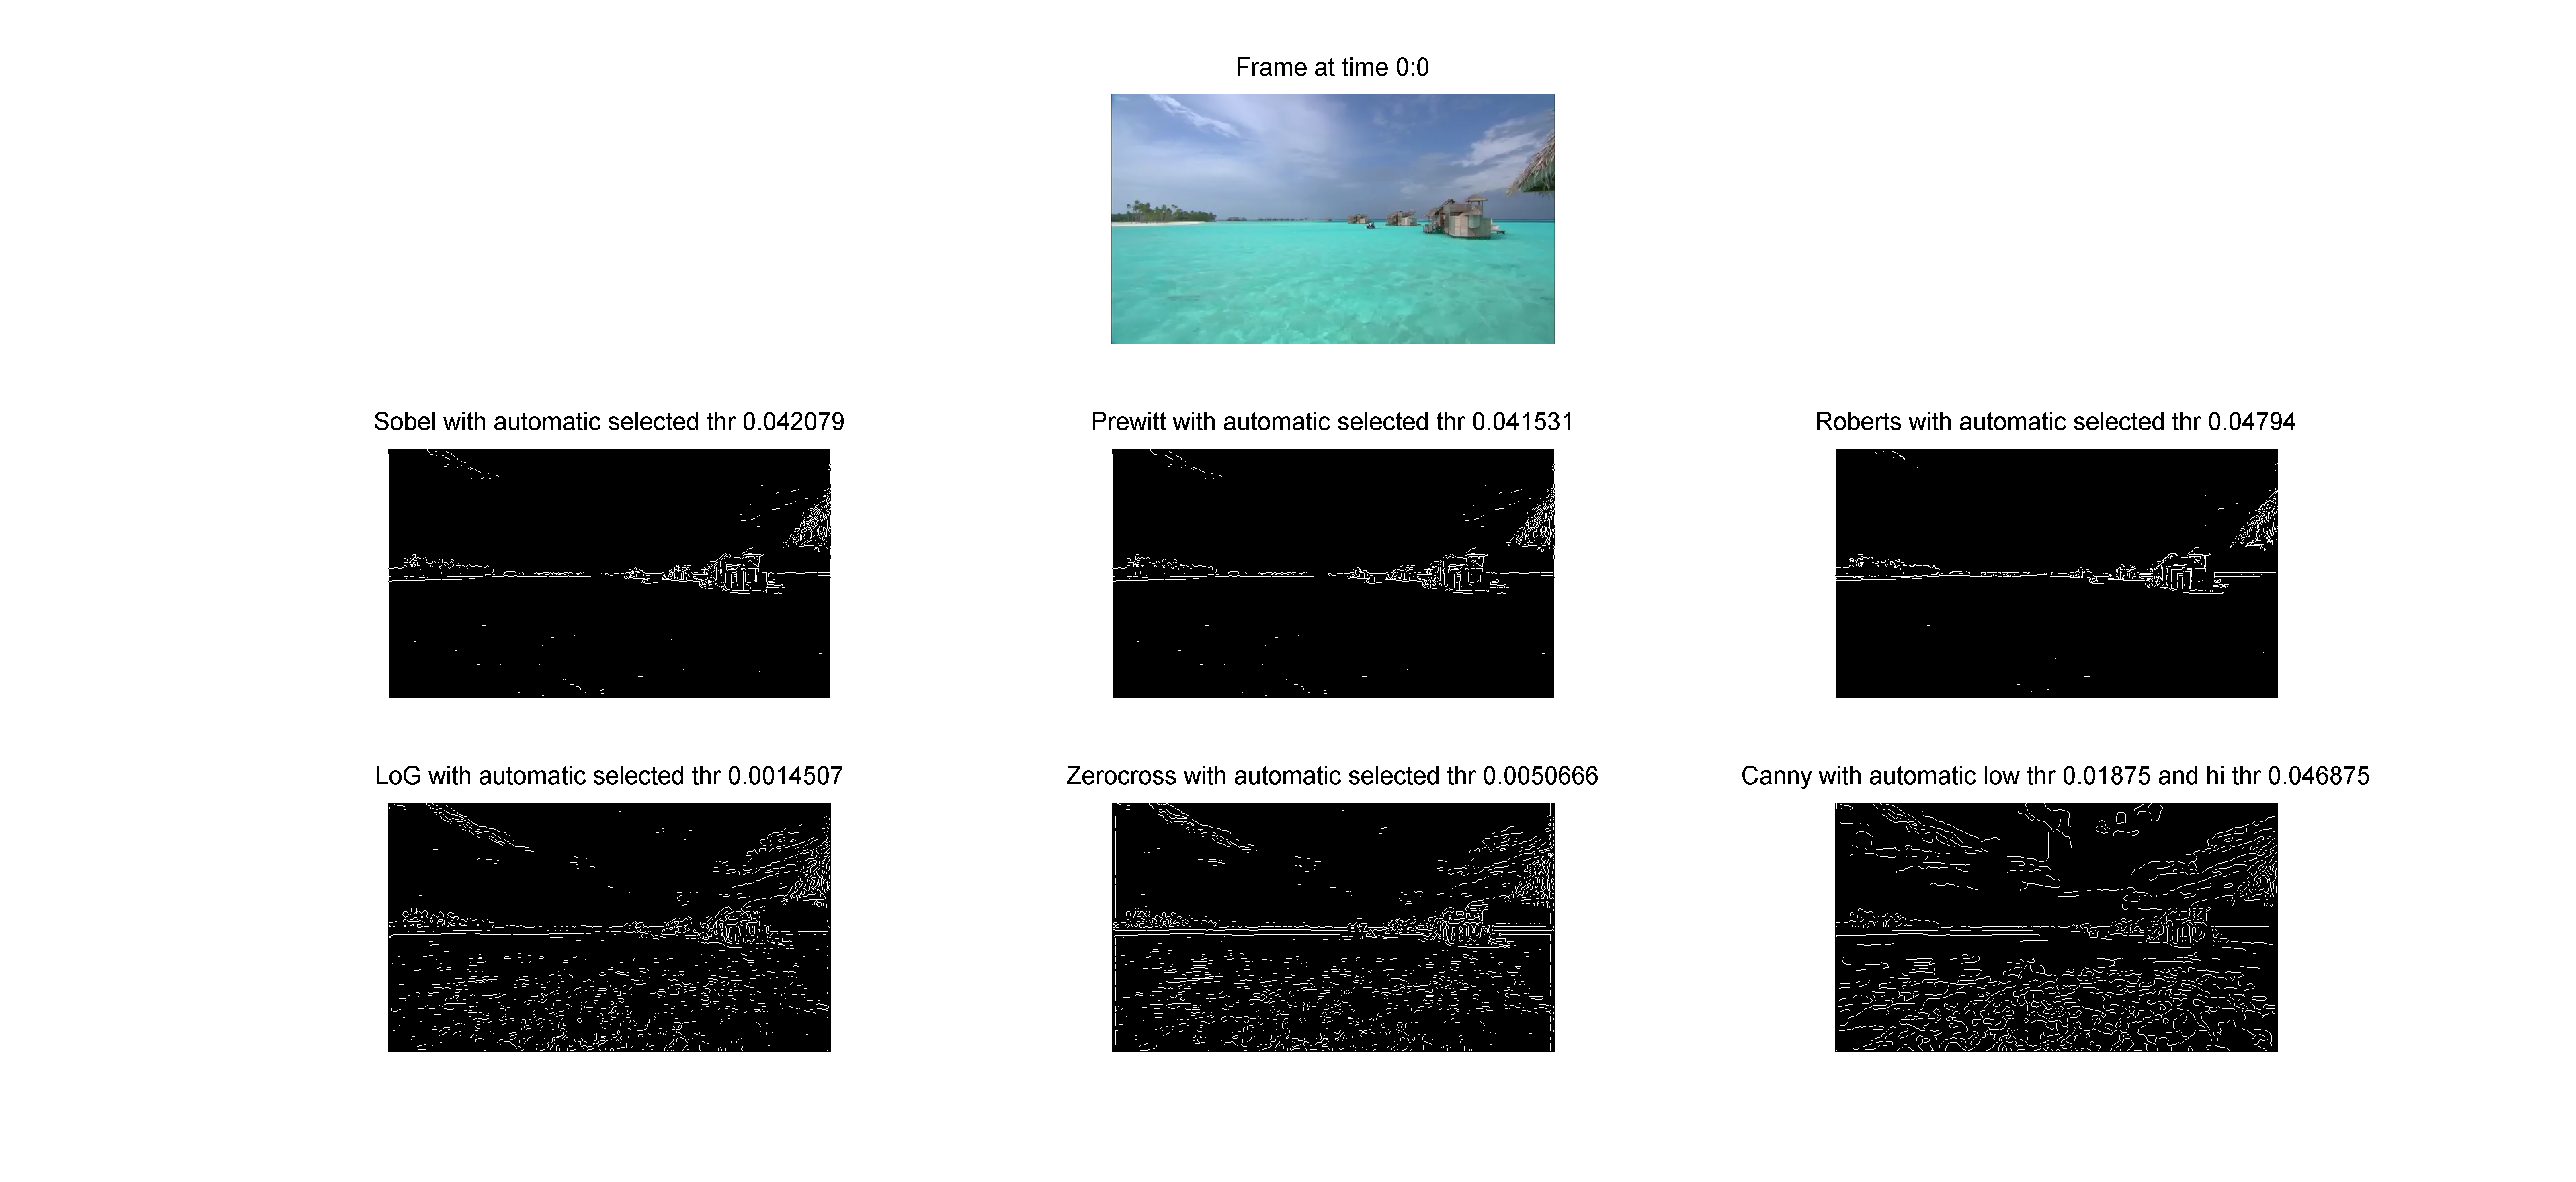
\includegraphics[width=\textwidth]{./img/ex2/comparison_0_0.png}
  \caption{Comparison of edge detectors at time 0:0}
  \label{fig:firstcomparison}
\end{figure}

\begin{figure}[!hbt]
  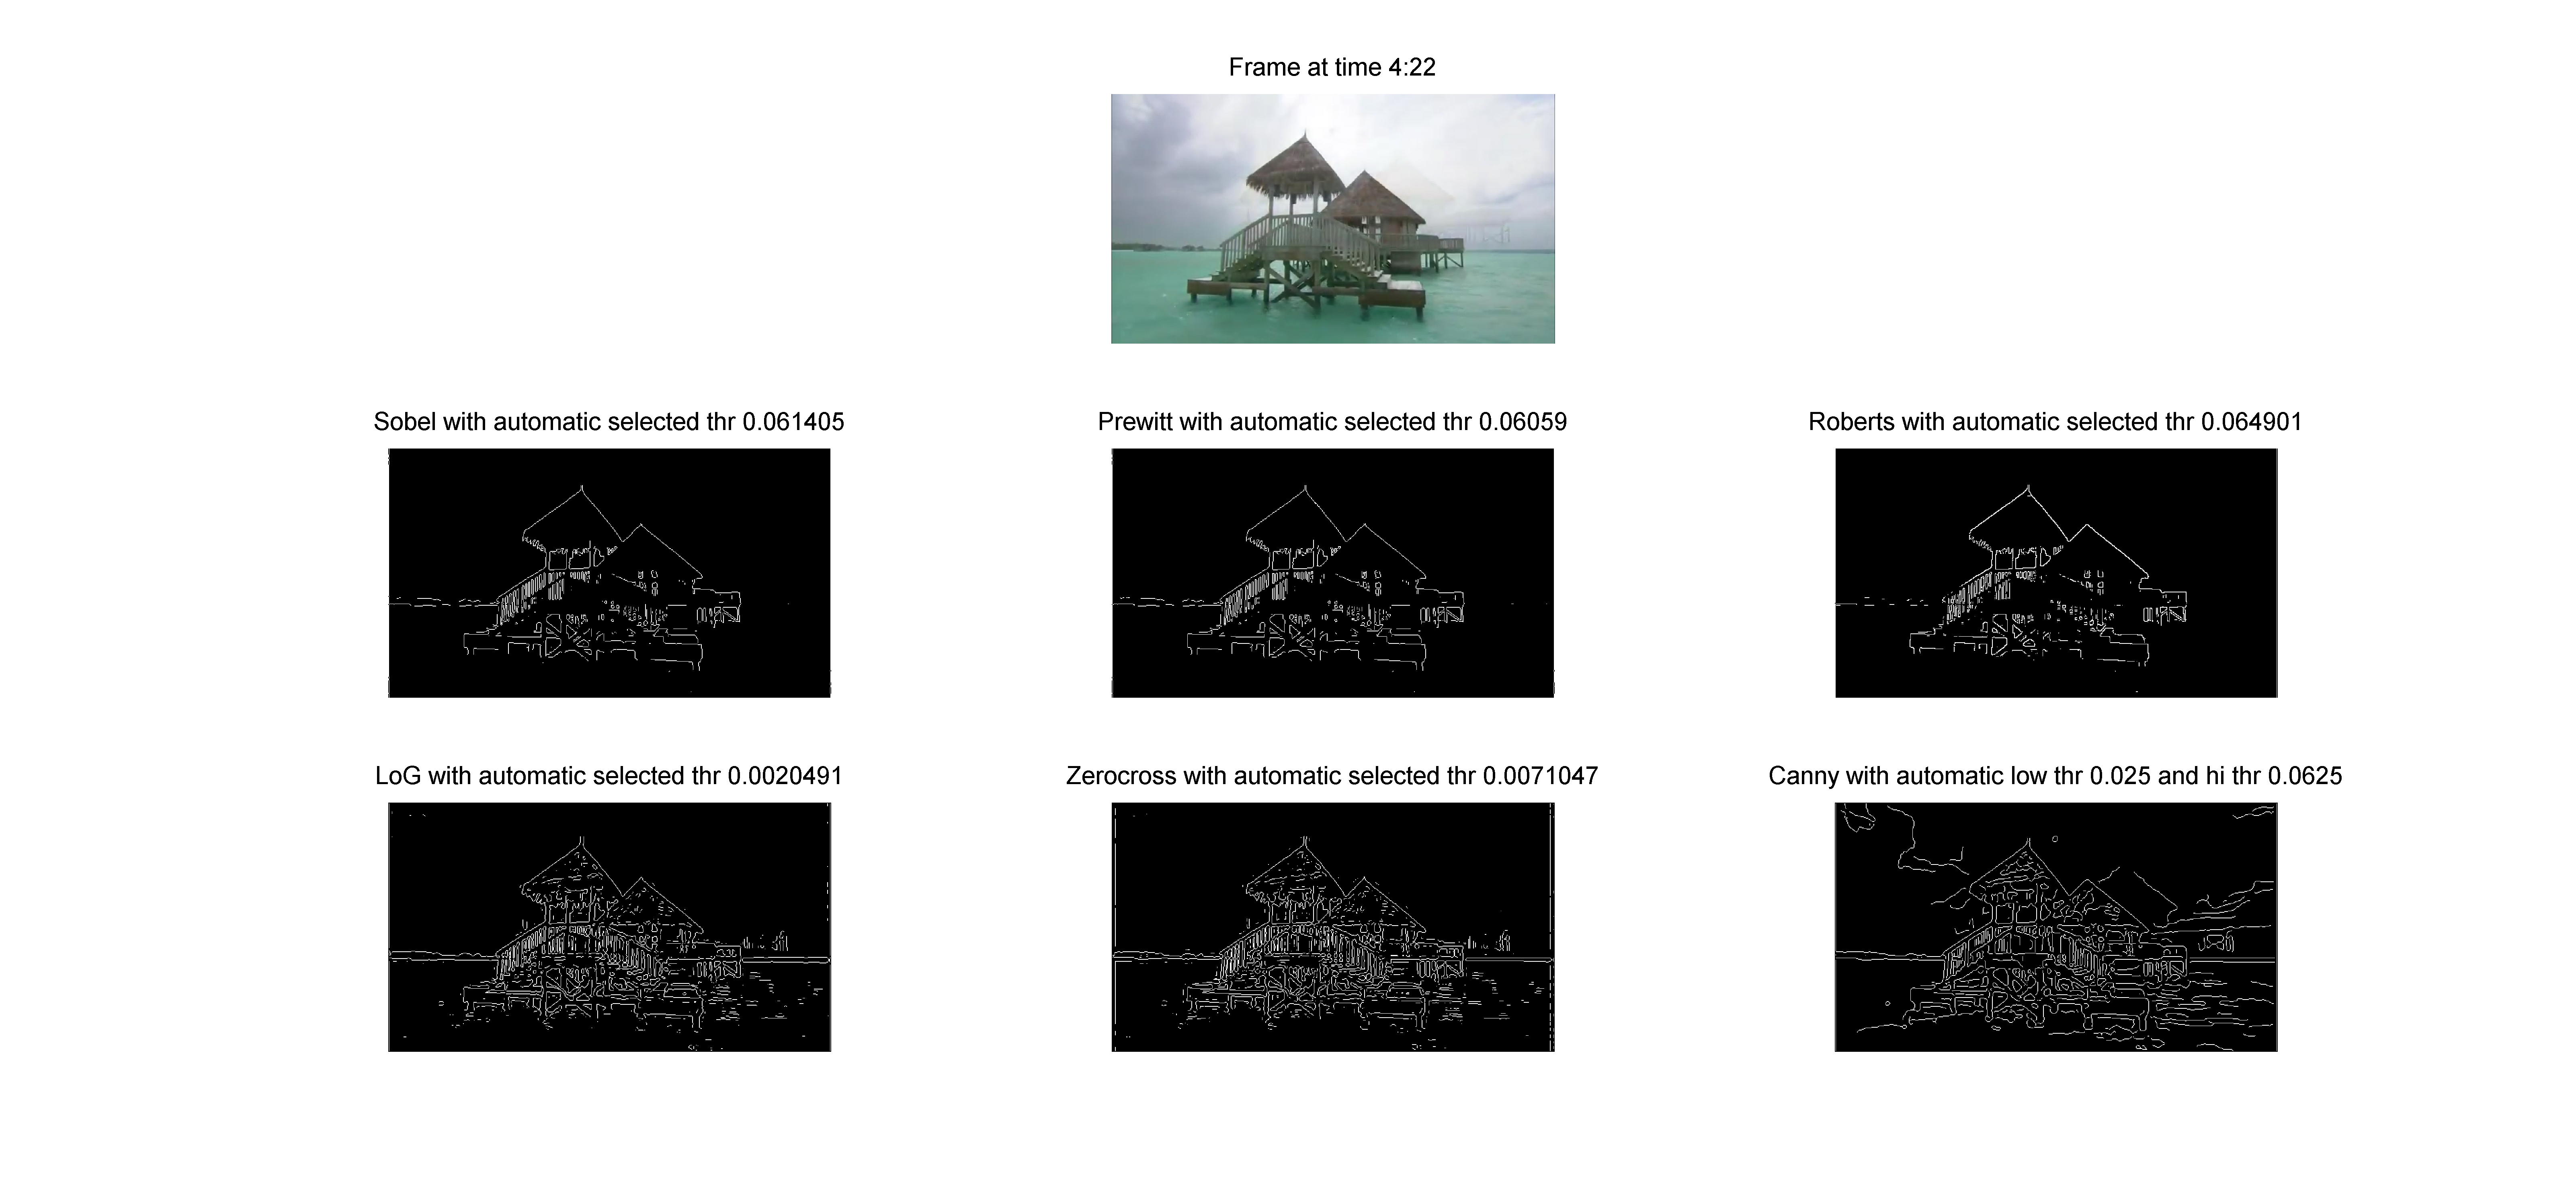
\includegraphics[width=\textwidth]{./img/ex2/comparison_4_22.png}
  \caption{Comparison of edge detectors at time 4:22}
  \label{fig:secondcomparison}
\end{figure}

\begin{figure}[!hbt]
  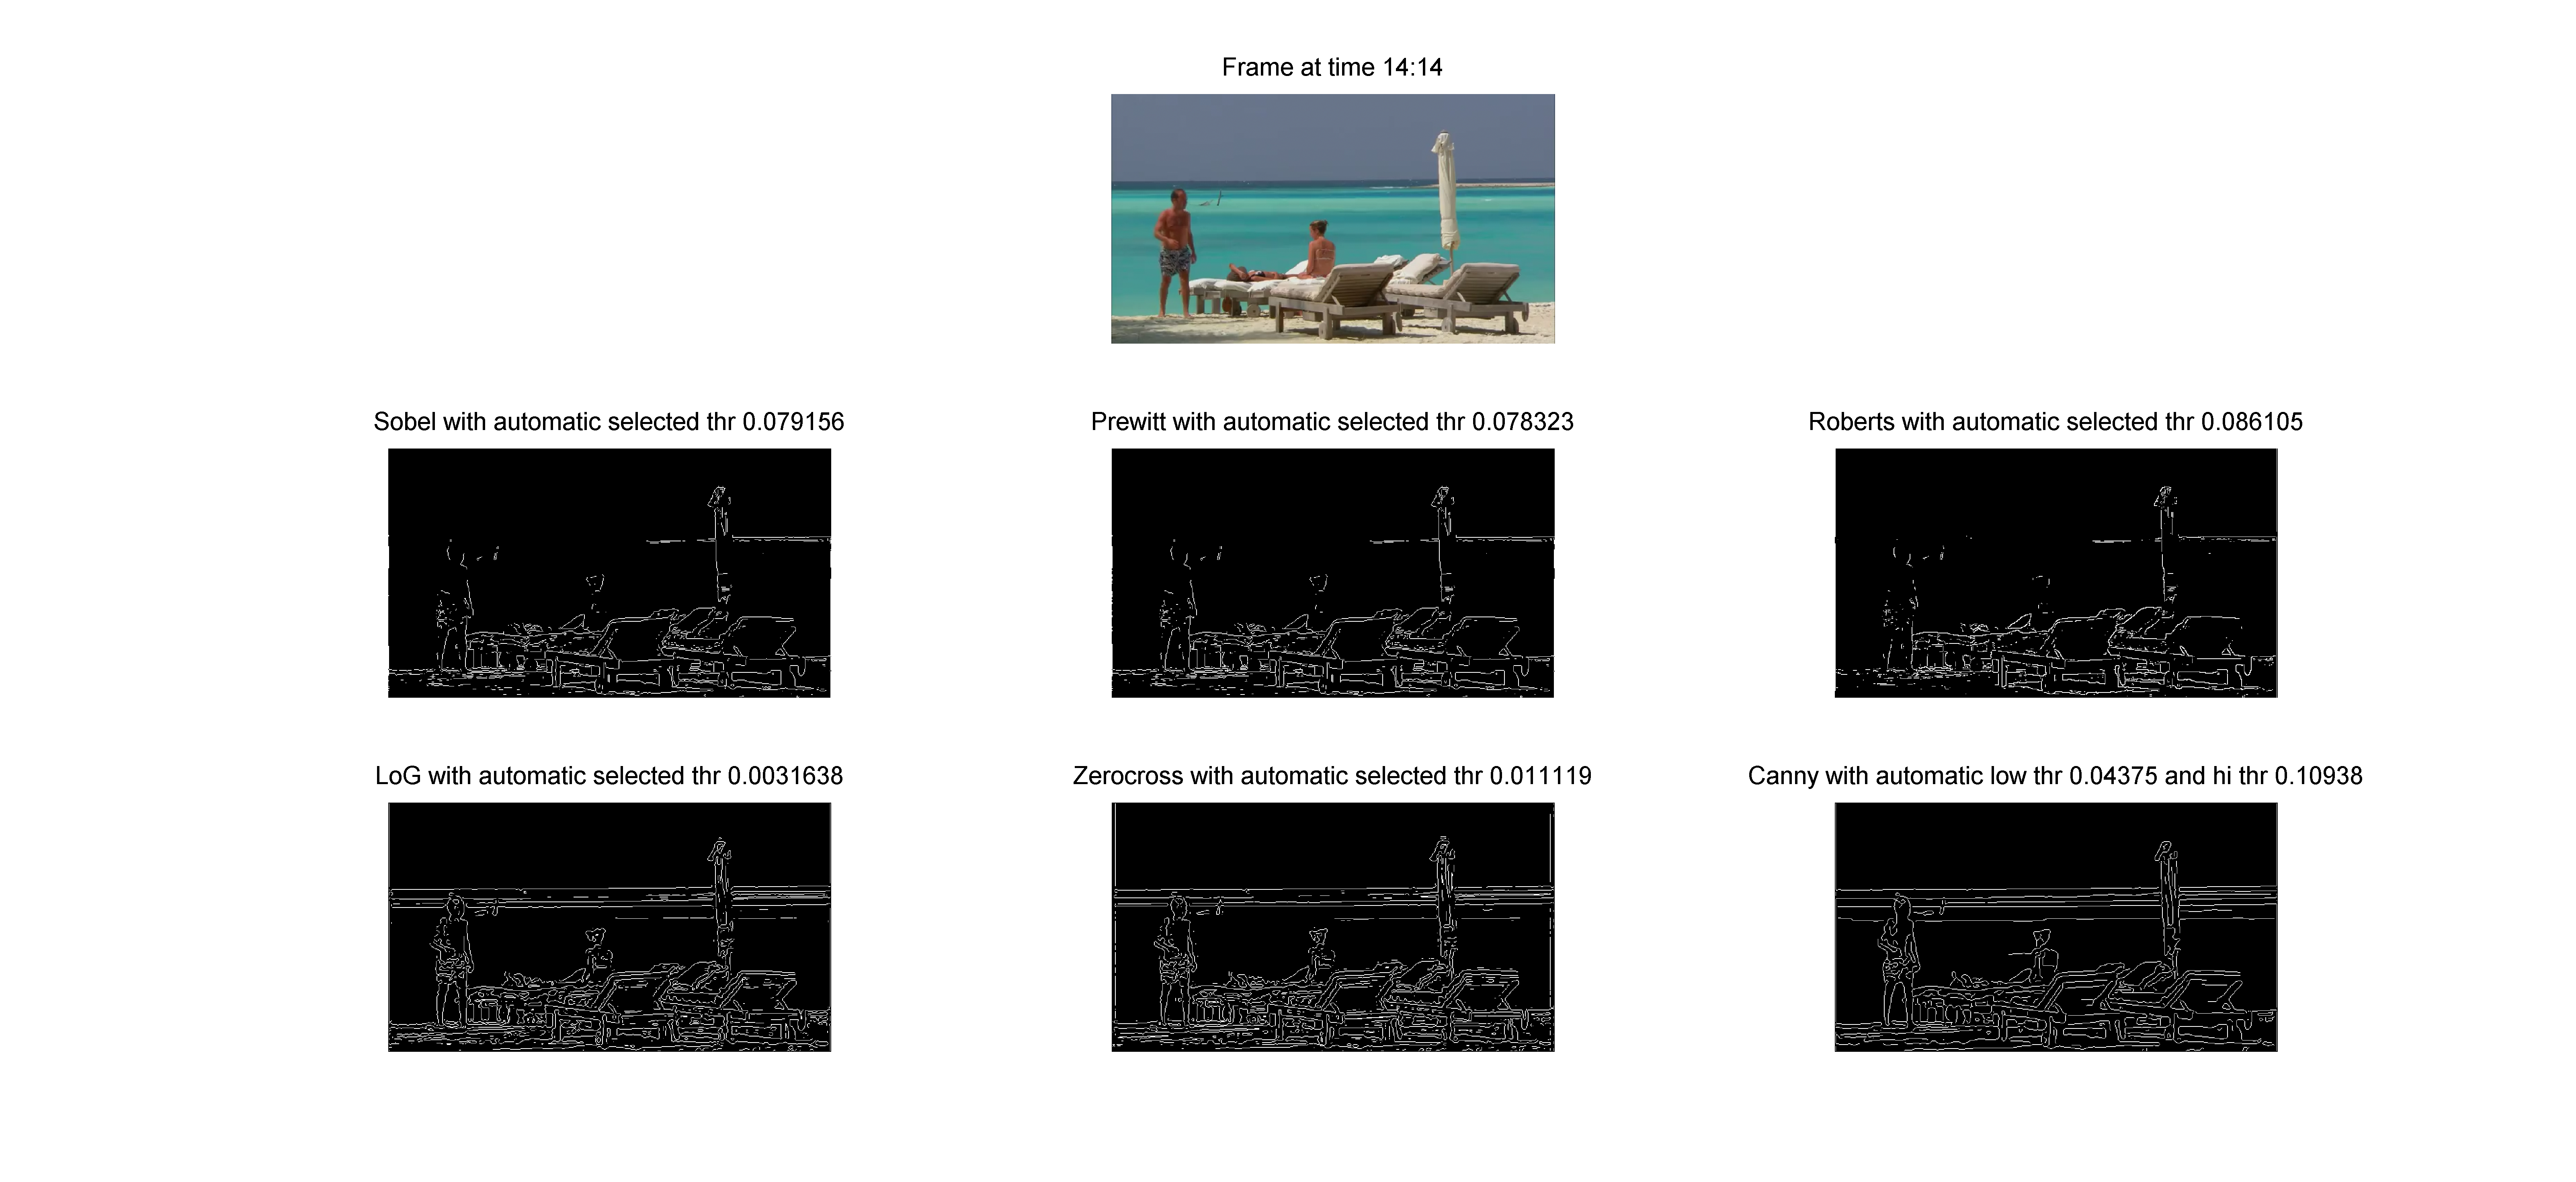
\includegraphics[width=\textwidth]{./img/ex2/comparison_14_14.png}
  \caption{Comparison of edge detectors at time 14:14}
  \label{fig:thirdcomparison}
\end{figure}

Again, which is the best detector depends upon the application. If we need
real-time efficiency, we would probably prefer Sobel, Prewitt or Roberts
(maybe even LoG or Zero-cross). If we can afford to
spend some time to process the frames beforehand, Canny would yield very good
results. For the particular case of this video, where all the frames have the same
resolution, similar amount of noise and similar color distributions and shapes, it
could be a good idea to tweak the parameters for a particular method. However,
we have found that letting the detector choose the thresholds automatically is
a good compromise between adaptability and quality. This is specially true in
videos where there are abrupt changes of scenes among different sections.